% !TEX TS-program = lualatex

% required for TexXstudio, an alternative is to change the default bibliography tool 
% in TeXstudio settings (Options > Configure TeXstudio > Build > Default Bibliography Tool)
% !BIB TS-program = biber

\documentclass[a4paper,11pt]{article}

\usepackage{geometry}
\geometry{left=20.00mm, right=15.00mm, top=20.00mm, bottom=20.00mm}

% this is to get rid of 'Overfull \hbox...' errors
\usepackage{microtype}

% ------------------------------------------------------------------------------
% Title
% ------------------------------------------------------------------------------

\title{\vspace{-1.5cm}Математический анализ и линейная алгебра \\
Домашнее задание №3}
\author{Дмитрий Донецков (ddonetskov@gmail.com)}
\date{\today}

% ------------------------------------------------------------------------------
% LUA
% ------------------------------------------------------------------------------

% \usepackage{luacode}

% ------------------------------------------------------------------------------
% Graphics
% ------------------------------------------------------------------------------

\usepackage{graphicx}

% https://www.sharelatex.com/learn/Pgfplots_package
\usepackage{pgfplots}
\pgfplotsset{compat=1.15}\usepgfplotslibrary{fillbetween}

\usepackage{wrapfig}

% ------------------------------------------------------------------------------
% Figures
% ------------------------------------------------------------------------------

\usepackage{subcaption}         % subcaptions in figures

% ------------------------------------------------------------------------------
% Tables
% ------------------------------------------------------------------------------

\usepackage{multirow}           % spanning columns across multiple rows
\usepackage{makecell}           % allows different formats inside cells

\renewcommand\theadalign{bc}
\renewcommand\theadfont{\bfseries}
\renewcommand\theadgape{\Gape[4pt]}
\renewcommand\cellgape{\Gape[4pt]}

% ------------------------------------------------------------------------------
% Math (Additional Support)
% ------------------------------------------------------------------------------

\usepackage{amsmath,amsfonts,amssymb,amsthm,mathtools}     % AMS
\usepackage{cancel}             % four different modes of striking through
\usepackage{dsfont}
\usepackage{icomma}             % Smart comma: $0,2$ --- число, $0, 2$ --- перечисление
%\usepackage{nicefrac}          % looks like xfrac is better maintained
\usepackage{physics}            % implementation of \abs and \norm
\usepackage{xfrac}

\DeclareMathOperator*{\D}{\mathbb{D}}   % the dispersion symbol
\DeclareMathOperator*{\E}{\mathbb{E}}   % the expectation symbol

\DeclareMathOperator*{\N}{\mathbb{N}}   % the set of natural numbers
\DeclareMathOperator*{\R}{\mathbb{R}}   % the set of real numbers
\DeclareMathOperator*{\Z}{\mathbb{Z}}   % the set of integers

% e = 2.71...
\newcommand{\e}{\mathrm{e}}

% sign of independence
% \vDash can also be used instead of \models
% \raisebox{}{} is required for vertical alignment
\newcommand{\independent}{\raisebox{0.05em}{\rotatebox[origin=c]{90}{$\models$}}}

%\newcommand\independent{\protect\mathpalette{\protect\independenT}{\perp}}
%\def\independenT#1#2{\mathrel{\rlap{$#1#2$}\mkern2mu{#1#2}}}

% ------------------------------------------------------------------------------
% Russian Language (support thereof)
% ------------------------------------------------------------------------------

\usepackage[russian,english]{babel}	    % локализация и переносы

% ------------------------------------------------------------------------------
% Fonts 
% ------------------------------------------------------------------------------

\usepackage{fontspec}           % required to load Open Type, True Type fonts

\setmainfont{CMU Serif}
\setsansfont{CMU Sans Serif}
\setmonofont{CMU Typewriter Text}

%\setmainfont{Linux Libertine O} % Libertine covers Latin, Hebrew, Greek, and Russian
%\setmonofont{Courier New}

\usepackage{euscript}	          % Шрифт Евклид
\usepackage{mathrsfs}           % Красивый матшрифт

% ------------------------------------------------------------------------------
% Bibliography 
% ------------------------------------------------------------------------------

% Removed as it was not required.

% ------------------------------------------------------------------------------
% Bookmarking, citing, URL's
% ------------------------------------------------------------------------------

% hyperref usually needs to be loaded last
\usepackage{hyperref}
\usepackage{url}
% \usepackage[dvipsnames]{xcolor}

\hypersetup{
    colorlinks=true,
    linkcolor=blue,
    filecolor=red,      
    urlcolor=blue,
}

\urlstyle{same}

% ------------------------------------------------------------------------------
% Various
% ------------------------------------------------------------------------------
\usepackage{listings}
\lstset{showstringspaces=false}

% ------------------------------------------------------------------------------
% Document
% ------------------------------------------------------------------------------

\begin{document}

\maketitle

\section{Задачи}

\subsection{Задача 1}

Данная задача была ранее решена, как задача 8 задания 2.

\subsection{Задача 2}

Параметрическое уравнение касательного вектора: $r'(t) = (1, -2\sin 2t, 2\cos 2t)$.

Точке $(\pi, 1, 0)$ соответствует значение $t = \pi$, касательный вектор в данной точке  принимает значение $r'(\pi) = (1, 0, 2)$. 

Точке $(\sfrac{\pi}{2}, -1, 0)$ соответствует значение $t = \sfrac{\pi}{2}$, касательный вектор в данной точке принимает значение $r'(\sfrac{\pi}{2}) = (1, 0, -2)$.

Кривая $r(t)$ и касательные вектора отображены на \ref{fig:task2}. Данную кривую можно представить, как спираль вокруг оси $Ox$ с периодом $\pi$.

\begin{figure}[h!]
  \centering
    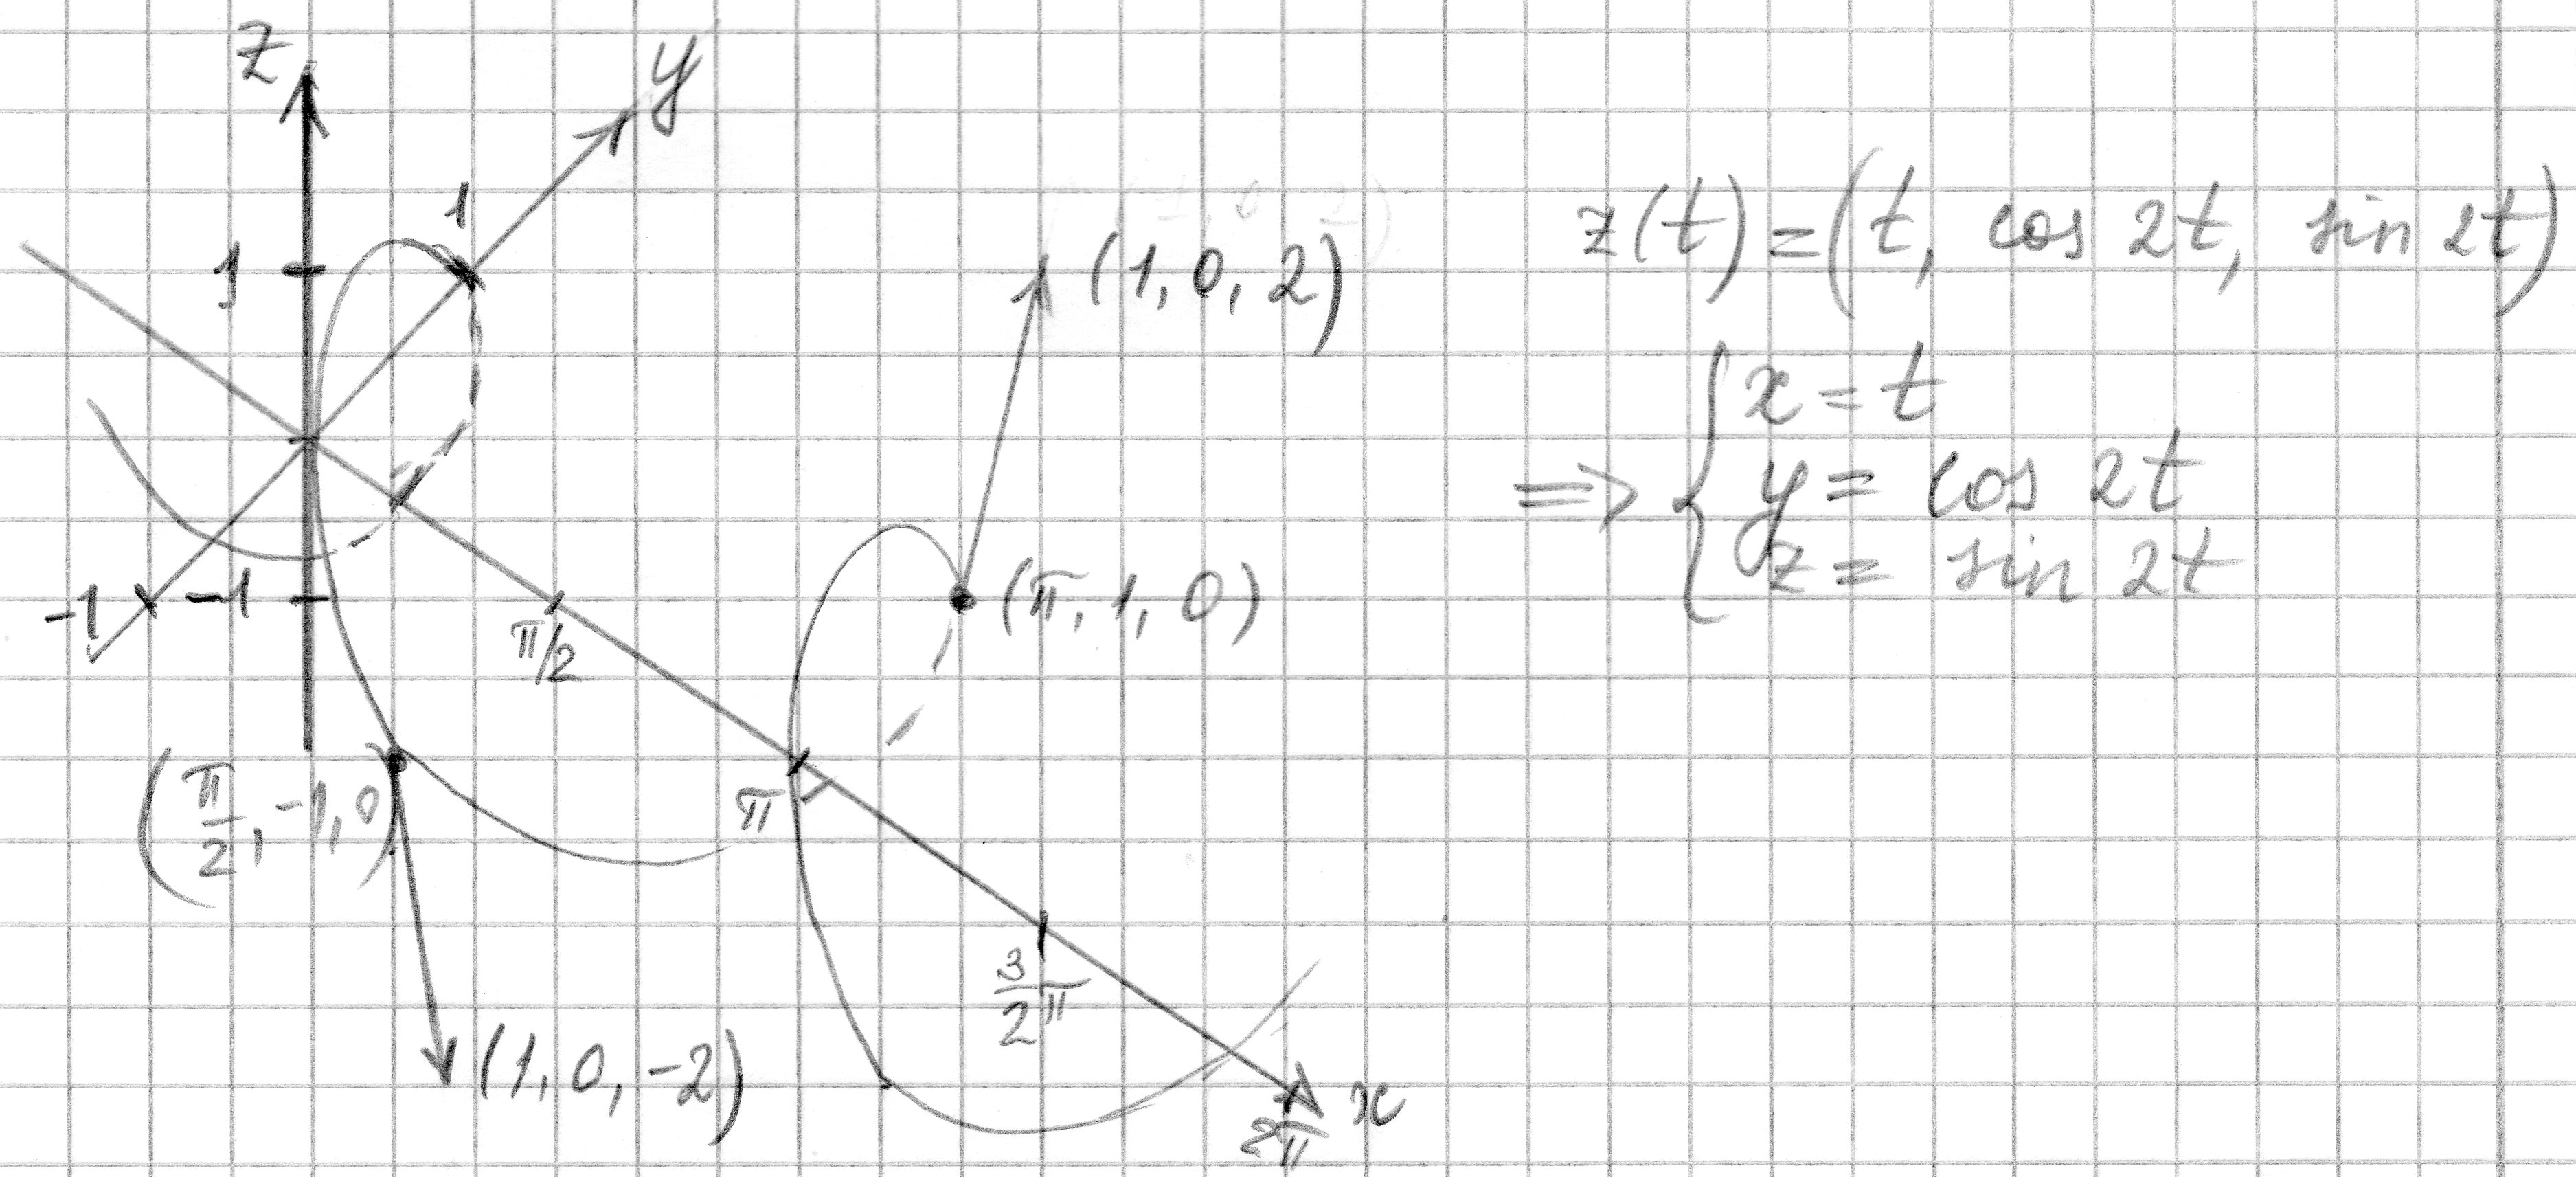
\includegraphics{images/task2.jpg}
  \caption{Эскиз кривой $r(t) = (t, \cos 2t, \sin 2t)$ и касательных векторов к ней.}
  \label{fig:task2}
\end{figure}

\newpage

\subsection{Задача 3}

См. рис. \ref{fig:task3}. Область определения функции - $\R^2$, область значений - $[4, +\infty)$.

\begin{figure}[h!]
  \centering
    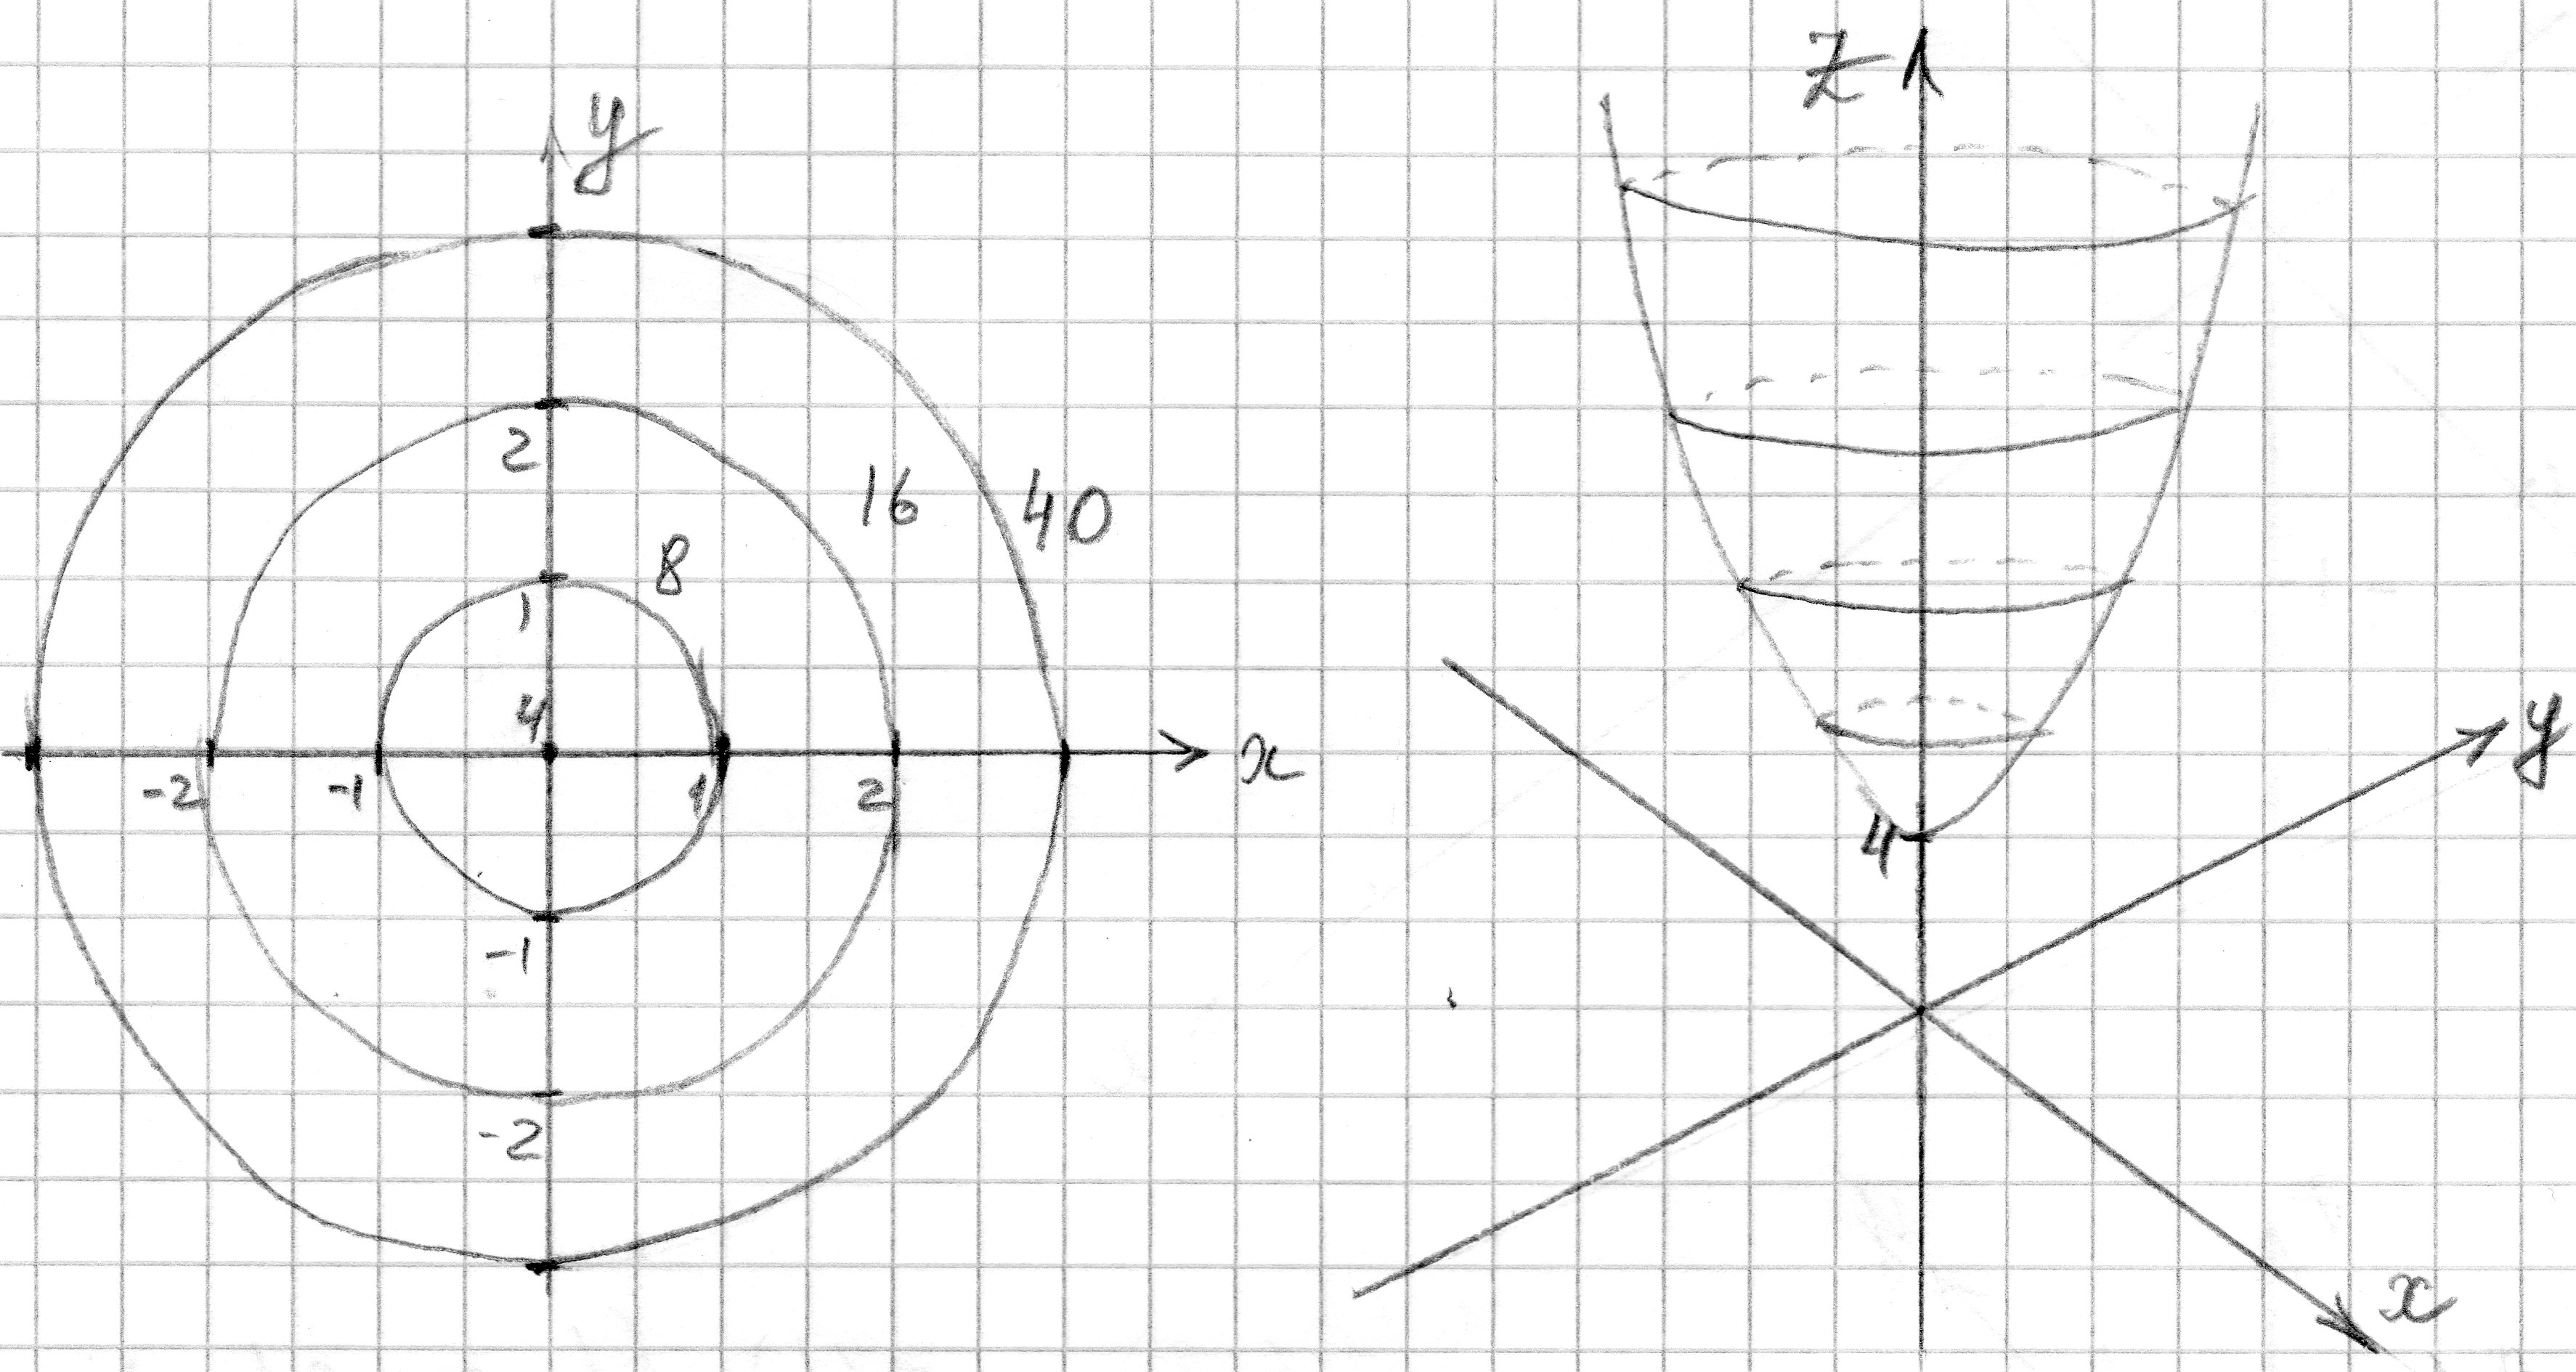
\includegraphics{images/task3.jpg}
  \caption{Линии уровня $f(x,y) = 4x^2 + 4y^2 + 4$ и эскиз её поверхности.}
  \label{fig:task3}
\end{figure}

\subsection{Задача 4}

Градиент функции $\nabla f(4, 6)$ показан на рис. \ref{fig:task4}. Он направлен в сторону роста значений функций и перпендикулярно линии уровня функции в заданной точке.

\begin{figure}[h!]
  \centering
    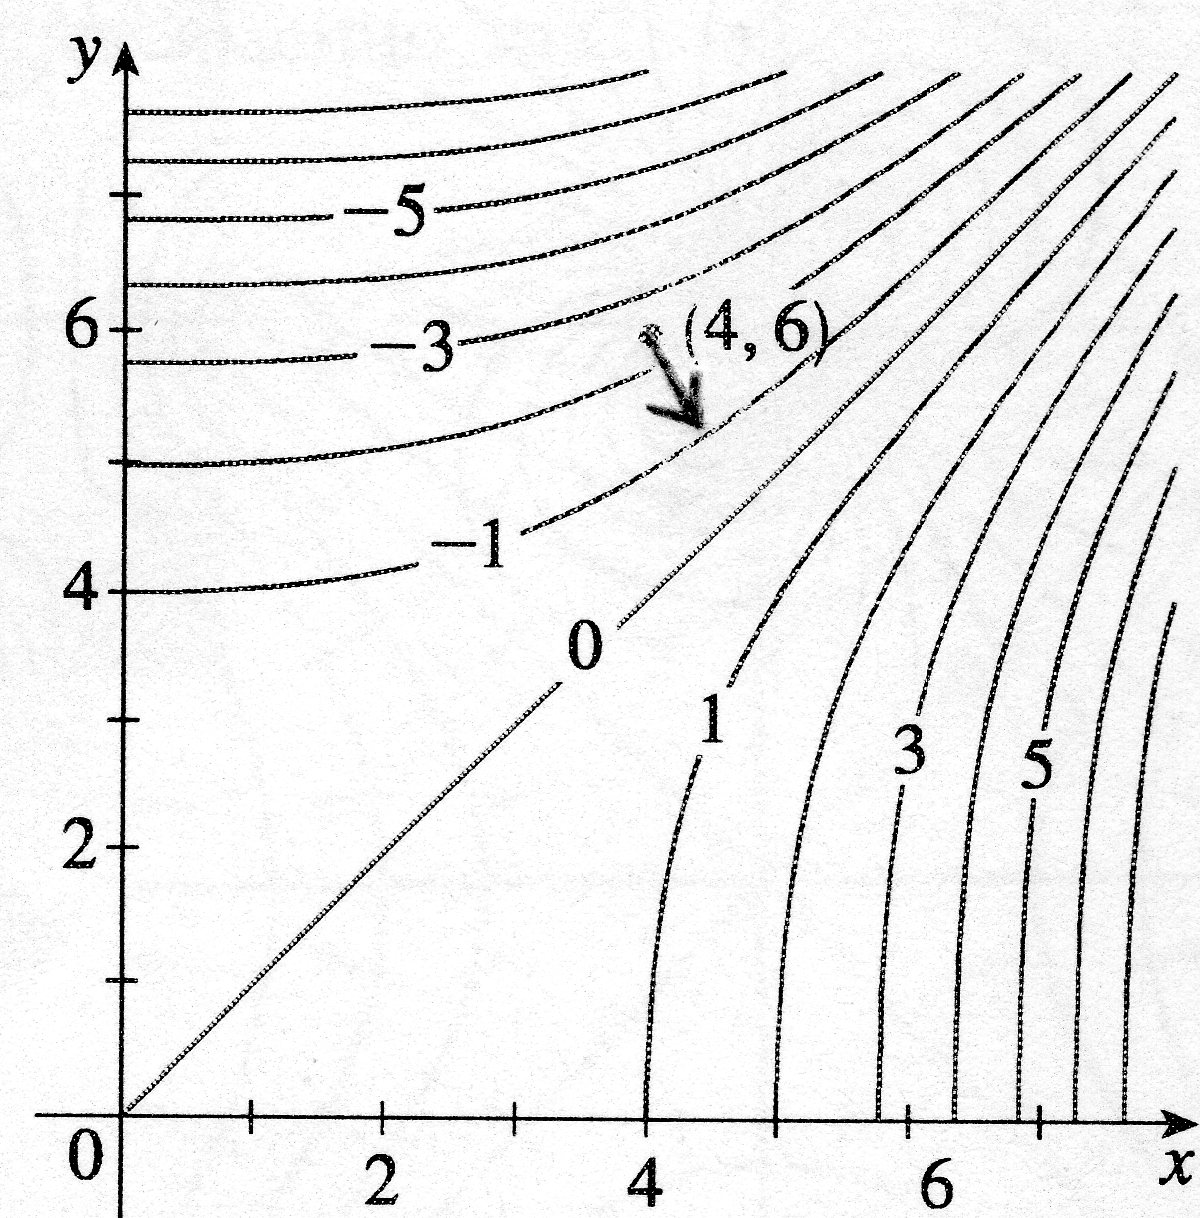
\includegraphics{images/task4.jpg}
  \caption{Заданные линии уровня с отмеченным градиентом}
  \label{fig:task4}
\end{figure}

\subsection{Задача 5}

Найдём частные производные функции $f(x,y) = x^4 + y^4 -4xy + 2$:

\begin{minipage}{0.4\linewidth}  
\begin{align*}
f_X & = 4x^3 -4y, \\
f_Y & = 4y^3 -4x,
\end{align*}
\end{minipage}  
\begin{minipage}{0.3\linewidth}  
\begin{align*}
f_{XX} & = 12x^2, \\
f_{YY} & = 12y^2,
\end{align*}
\end{minipage}
\begin{minipage}{0.3\linewidth}
\begin{align*}
f_{XY} & = -4, \\
f_{YX} & = -4.
\end{align*}
\end{minipage}

\vspace{1em}

Определим в каких точках градиент $\nabla f(x, y) = (4x^3-4y, 4y^3 -4x)$ равен (0, 0):

\begin{align*}
\begin{cases*}
4x^3 - 4y = 0,\\
4y^3 - 4x = 0.
\end{cases*}
\quad \Rightarrow \quad 
\begin{cases*}
x^3 - y = 0,\\
y^3 - x = 0.
\end{cases*}
\quad \Rightarrow \quad 
\begin{cases*}
x^3 - \sqrt[3]{x} = 0,\\
y^3 - \sqrt[3]{y} = 0.
\end{cases*}
\end{align*}

Корнями данной системы уравнений являются точки $A = (0, 0), B = (1, 1)$. Это точки, которые могут быть как точками экстремума, так и седловыми точками. Для определения характера точек воспользуемся достаточным условием экстремума. Вычислим значения вторых частных производных и определителя функции $D = f_{XX}f_{YY}-f_{XY}^2 = 144x^2y^2 - 16$ в данных точках:

\begin{center}
\begin{tabular}{|c|c|c|c|}
\hline 
Точка & A = (0,0) & B = (1,1) \\ 
\hline 
$f_{XX}$ &   0 &  12 \\ 
$f_{YY}$ &   0 &  12 \\ 
$f_{XY}$ & -16 & -16 \\ 
\hline 
D & -16 & 128 \\ 
\hline 
\end{tabular} 
\end{center}

Исходя из значений детерминанта и вторых частных производных, точка B является точкой минимума. С точкой A возникла неопределенность, т.к. $D = 0$ в данной точке.

Посмотрим значения самой функции в окрестности такой точки. Так, для малых $(\varepsilon, \delta)$:

\begin{align*}
f(\varepsilon, 0) & = \varepsilon^4 + 2 > 0, \\
f(0, \delta)   & = \delta^4 +2 > 0.
\end{align*}

Т.е. функция в самой точке принимает значение $f(0,0) = 2$, а её окрестностях - значения больше, чем 2, то точка A является точкой минимума.

\subsection{Задача 6}

Данная задача была ранее решена, как задача 6 задания 2.

\subsection{Задача 7}

Данная задача была ранее решена, как задача 7 задания 2.

\end{document}
